\chapter{結論}
本論文では



記法メモ\\
test\cite{babi} \cite{memory_net} \cite{ntm} \cite{dnc} \cite{cslm} \cite{rrnn} \cite{simple_rel}
\cite{sam} \cite{gat} \cite{working2mem}
Wavenet\cite{oord2016wavenet}は
音声波形を時系列データとして自己回帰モデルで学習することによって,人間の声のような自然な音声を生成することができる.
時点$t$における観測値を$x_t$,$\bm{x} = \left\{ x_1, ..., x_T \right\}$を観測値の全体集合とする.このとき,波形の同時確率は 条件付き確率の積として
以下のよう表現される.
\begin{equation}
	p(\bm{x}) = \prod_{t=1}^T p(x_t | x_1, ..., x_{t-1})
\end{equation}

つまり,$x_t$は前時点の全てにおけるサンプルに条件づけられる.



図\ref{fig:ccl}に因果的畳み込み層のスタックを示す.

\begin{figure}[t]
	\centering
	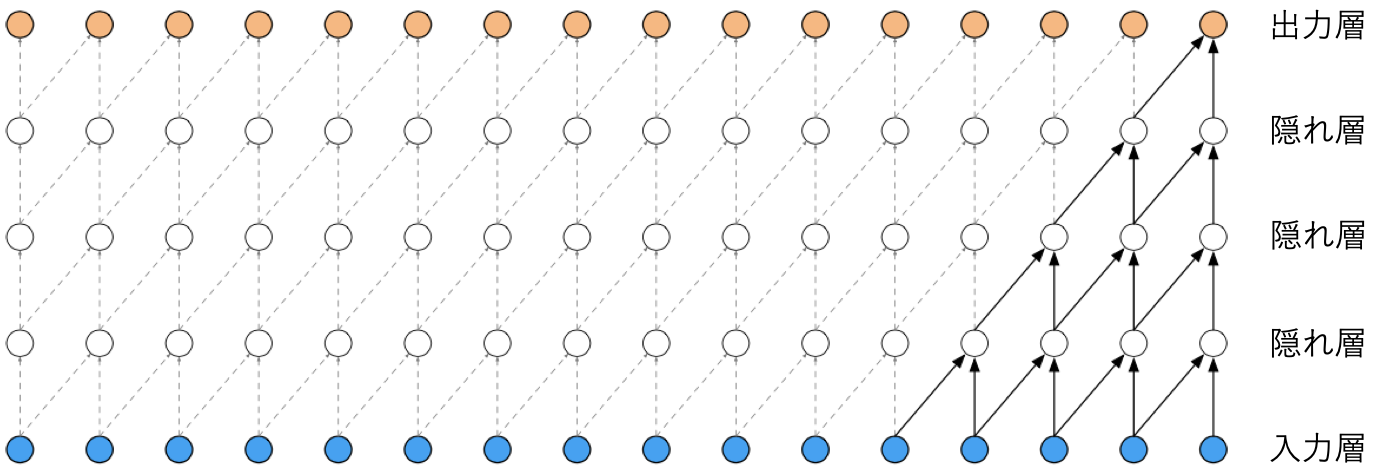
\includegraphics[width=\linewidth]{./figure/ccl.png}
	\caption{因果的畳み込み層}
	\label{fig:ccl}
\end{figure}

\cite{juang1991hidden}は.

今後の課題を以下に挙げる.
\begin{itemize}
	\item の向上
	\par
	必要がある.
	\item への応用
	\par
	を行いたい.
	\newpage
	\item の改善
	\par
	今後,取り組みたい.
\end{itemize}

しかしRMCの追加によって学習にかかる時間が増加し、
学習の高速化

samは項目メモリ内容の間の関係情報を関係メモリに保存する際に、線形変換で圧縮=項目の抽出?をしている。
入力が大きすぎて冗長なのが問題の場合、オートエンコーダのように圧縮・抽出したり、項目メモリ→関係メモリの部分のために読み出し操作をもう一つ実装するとよいかも
でかすぎたか RMCはもともと1ベクトルを入力 無理やり拡張した クエリとの齟齬も

上の実験とは関係なく、実験2の考察を踏まえて、今後修士で試す予定の改善のこともいくつか考えていますがこれらは結論に書く形になると思います。ひとまず以下に箇条書きします
\\関係メモリをRMCではなくSAMにしてみる。もともとRMCは1メモリモデルで入力がベクトルなので、無理に拡張するよりこちらのほうがいいかも
\\SAMや\cite{working2mem}〜のような2メモリモデルを見る限り、関係メモリから項目メモリの内容を復元する操作がある。今は項目→関係の一方向だけど逆も入れてメモリが相互作用できるようにする
\\samは項目メモリ内容の間の関係情報を関係メモリに保存する際に、線形変換で圧縮=項目の抽出?をしている。
入力が大きすぎて冗長なのが問題の場合、オートエンコーダのように圧縮・抽出したり、項目メモリ→関係メモリの部分のために読み出し操作をもう一つ実装するとよいかも
\\似た話としてgraph attentionを利用して時間的・コサイン類似度的に近い項目に重み付けをしたセルフアテンションをかける。この結果を関係メモリに保存する(rmc,SAMとは異なる構造の関係メモリになる)

babi 

また現在の提案ネットワークにおける情報の受け渡しは項目メモリから関係メモリの方向に限定されている。
一方で、既存の2メモリモデルには関係メモリから項目メモリへと情報を渡す経路も存在する。
STMには関係メモリが関連する項目を復元し、項目メモリに改めて書き込む操作が実装されている。
[LTD]は長期記憶と作業記憶からなる2メモリモデルであるが、一方の読み出しベクトルを入力に結合しもう一方の読み書き操作で利用する。
提案ネットワークにもこのような経路を導入し、2つのメモリの連携を強化する改善が考えられる。
Nth-farthestタスクにおいては関係メモリのみを持つRMCにより十分な精度を達成することが示されている。
一方で\cite{sam}では、最短経路や最小全域木の探索タスクや同論文で提案されたRARタスクにおいては2つのメモリの存在が性能を向上させることが示されている。
このようなタスクにおいて、上記の改善が提案ネットワークの性能を改善させる可能性が考えられる。

時間順序に着目すると DNCのlink matrix
\ref{chap:link-matlix}
